%!TEX root = ../../main.tex

Sabe-se que algoritmos de AM necessitam de quantidade significantiva de dados, preferencialmente sem muitos ruídos, para serem utilizados de forma a obter um modelo que possua bom desempenho \cite{marsland}. Levando isto em conta e com vistas a adequar os dados disponíveis com a tarefa de aprendizado considerada, uma etapa de pré-processamento fez-se necessária, cujos passos são descritos a seguir.

Primeiramente foi necessário realizar a adaptação das imagens individuais para as imagens compostas, conforme apresentado anteriormente no esquema da Figura \ref{fig:esquema-solucao}. Para isto, foi feita a combinação de cada assinatura genuína de um autor com suas diferentes versões originais, produzindo uma nova imagem para cada caso, a qual associou-se o rótulo de autêntica. Após esta etapa, também foram combinados os exemplos genuínos com suas respectivas versões forjadas, aos quais foi associado o rótulo de forjado. Todas as imagens obtidas dessas combinações serão utilizadas como exemplos para o processo de treinamento, validação e teste do modelo proposto.

Para preservar a referência aos autores e ids de suas assinaturas, os nomes dos arquivos passaram a conter tais informações. Entretanto, ressalta-se que os modelos de CNNs não terão acesso a este dado (nome do arquivo). Ele serve de referência apenas para verificar a procedência do exemplo.

O processo de combinação das imagens de cada um dos exemplos foi realizado em três etapas. Na primeira etapa, ambas as imagens foram redimensionadas para um tamanho de $256 \times 256$ \emph{pixels}. Em seguida, as imagens foram concatenadas verticalmente com a intenção de formar uma única imagem de $256 \times 512$ \emph{pixels}. Por fim, a imagem resultante foi redimensionada novamente em um tamanho de $256 \times 256$ \emph{pixels} e transformada para um espaço de cores em escala de cinza, com a intenção de padronizar todos os exemplos.

Ao concluir o processo anterior, necessitou-se então a realização da partição dos exemplos conforme o método \emph{holdout} e, com vistas a evitar que fossem apresentadas as assinaturas de um mesmo indivíduo a um modelo durante as etapas de treinamento e teste, foram adotadas duas abordagens diferentes. Na primeira destas, chamada de abordagem A, decidiu-se evitar o aparecimento apenas dos exemplos forjados de um mesmo autor em duas partições diferentes, sendo assim, os exemplos autênticos foram distribuídos conforme o método previamente especificado, enquanto que os exemplos forjados foram separados seguindo os seguintes critérios:

% Ao concluir a etapa anterior, realizou-se então, nos exemplos autênticos, a partição \emph{holdout} previamente especificada. Porém, esta mesma ideia não podia ser realizada nos exemplos forjados, pois culminaria na apresentação de uma mesma falsificação na etapa de treinamento e de teste, favorecendo a sua detecção. Em um cenário prático de eventual utilização da solução proposta, o modelo construído já terá sido treinado e será requisitado a avaliar uma assinatura potencialmente forjada, mas nunca antes vista. Levando isto em consideração, a etapa de testes apenas incluirá assinaturas forjadas inéditas para o modelo. Para que isso fosse possível, alguns critérios de separação foram adotados:

\begin{itemize}
	\item Se uma assinatura autêntica possuía apenas um autor forjador, todos os exemplos forjados foram incluídos no conjunto de treinamento;
	\item Se uma assinatura autêntica possuía quatro autores forjadores, as assinaturas de três desses autores foram para o conjunto de treinamento e as remanescentes, pertencentes a apenas um autor, foram para o conjunto de teste;
	\item Se uma assinatura autêntica possuía cinco autores forjadores, as assinaturas de quatro desses autores foram para a etapa de treinamento e as remanescentes, pertencentes a apenas um autor, permaneceram na etapa de teste;
	\item Se uma assinatura autêntica possuía seis autores forjadores, as assinaturas de quatro desses autores foram para a etapa de treinamento e as assinaturas dos outros dois foram para a etapa de teste;
	\item Se uma assinatura possuía trinta ou mais autores forjadores, as assinaturas de dez desses autores foram para o conjunto de teste, três desses autores foram utilizados para o conjunto de validação e as assinaturas restantes foram remanejadas para o conjunto de treinamento.
\end{itemize}

Para a segunda abordagem, chamada de abordagem B, decidiu-se que não deveriam existir exemplos de um mesmo autor em duas partições diferentes, sendo estes exemplos forjados ou autênticos. Em um cenário prático de eventual utilização desta abordagem, o modelo construído já terá sido treinado e será requisitado a avaliar uma assinatura, tomando como referência uma assinatura autêntica de um autor nunca antes visto pelo modelo. Levando isto em consideração, a etapa de testes incluírá apenas exemplos de autores inéditos para o modelo. Para que isso fosse possível, a escolha da quantidade de autores para cada partição foi utilizada conforme o método \emph{holdout} especifidado anteriormente e, todos exemplos de dado autor, foram utilizados para a partição que lhe foi designada. Esta abordagem equivale ao método de avaliação considerado para os modelos submetidos à SigComp2009, sendo assim, seus resultados podem servir como forma de comparação às métricas coletadas durante esta competição \cite{icdar2009}. 

Os autores forjadores da abordagem A e todos os autores da abordagem B selecionados para estarem presentes em cada uma das partições foram escolhidos de forma pseudoaleatória. Dessa maneira, ressalta-se que os conjuntos de treino, teste e validação de ambas as abordagens são disjuntos no tocante aos autores forjadores.

Após o particionamento dos dados conforme especificado, tem-se o quantitativo dos dados de treino, validação e teste para cada uma das abordagens dispostos conforme Tabela \ref{tab:divisao-dados} e com proporcionalidades apresentadas nas Figuras \ref{fig:divisao-dados-a} e \ref{fig:divisao-dados-b}.

\begin{table}[h!]
	\centering
	\caption{Quantitativo de exemplos por finalidade na tarefa de aprendizado considerada e classe para cada abordagem.}
	\label{tab:divisao-dados}
	\resizebox{\textwidth}{!}{
	\begin{tabular}{c c c c c c}
		\toprule
		\multirow{2}{*}{\textbf{Conjunto}} & \multirow{2}{*}{\textbf{Tipo de Exemplo}} & \multicolumn{2}{c}{\textbf{Abordagem A}}  & \multicolumn{2}{c}{\textbf{Abordagem B}}\\ 
		 &  & \textbf{Nº de Exemplos} & \textbf{Proporção} & \textbf{Nº de Exemplos} & \textbf{Proporção}\\
		\midrule
		\multirow{2}{*}{Treinamento} & Autêntico & 9.374 & $54\%$ & 8.072 & $43\%$\\
    & Forjado & 8.131 & $46\%$ & 10.887 & $57\%$\\
     \midrule
		 \multirow{2}{*}{Validação} & Autêntico & 947 & $46\%$ & 1.179 & $37\%$ \\
     & Forjado & 1.134 & $54\%$ & 1.976 & $63\%$\\
		 \midrule
		 \multirow{2}{*}{Teste} & Autêntico & 2.257 & $27\%$ & 2.271 & $39\%$\\
     & Forjado & 6.119 & $73\%$ & 3.577 & $61\%$\\
		\bottomrule
	\end{tabular}}
\end{table}

\begin{figure}[h!]
\centering
\caption{Representação gráfica da proporção dos exemplos por classe e finalidade para as abordagens na tarefa de aprendizado considerada.}
\subfloat[Abordagem A.\label{fig:divisao-dados-a}]{%
	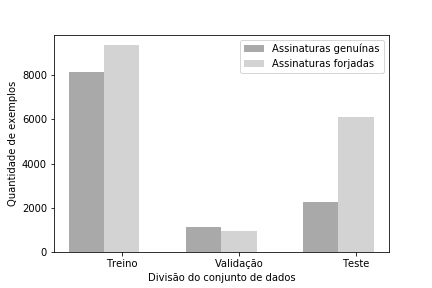
\includegraphics[width=0.49\textwidth]{imgs/new_approach}
}
\hfill
\subfloat[Abordagem B.\label{fig:divisao-dados-b}]{%
	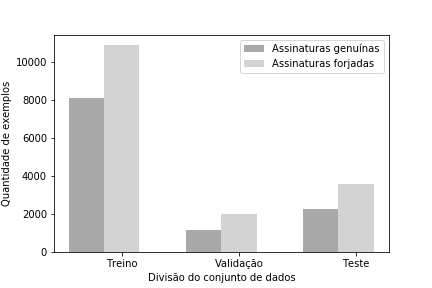
\includegraphics[width=0.49\textwidth]{imgs/approach_icdar}
}
\label{fig:dropout}
\end{figure}

Para a abordagem A, percebe-se que há uma certa desproporção entre as classes nas etapas de treino e validação. Na etapa de testes, esta diferença torna-se mais evidente e será refletida nas métricas de desempenho dos modelos. Quanto à abordagem B, tem-se uma notória desproporção nos conjuntos de validação e teste, isto devido à providência de considerar apenas a quantidade de autores e não a quantidade de exemplos durante a partição dos dados. Deste modo, esta diferença pode refletir tanto na parada precoce do treinamento quanto nas métricas de desempenho dos modelos.

Ao serem fornecidas para treinamento pelas CNNs em etapa posterior, todos os \emph{pixels} das imagens serão normalizados por meio de uma divisão por $255$, passando a residirem no intervalo $[0,1]$. Esta normalização é realizada em virtude das redes neurais que, em geral, aprendem mais eficientemente nestas condições \cite{chollet}. \todo{Inserir referência sobre melhor aprendizado das RNAS com valores entre 0 e 1.}
